%%%%%%%%%%%%%%%%%%%%%%%%%%%%%%%%%%%%%%%%%%%%%%%%%%%%%%%%%%%%%%%%%%%%
%% I, the copyright holder of this work, release this work into the
%% public domain. This applies worldwide. In some countries this may
%% not be legally possible; if so: I grant anyone the right to use
%% this work for any purpose, without any conditions, unless such
%% conditions are required by law.
%%%%%%%%%%%%%%%%%%%%%%%%%%%%%%%%%%%%%%%%%%%%%%%%%%%%%%%%%%%%%%%%%%%%

\documentclass[
  digital, %% This option enables the default options for the
           %% digital version of a document. Replace with `printed`
           %% to enable the default options for the printed version
           %% of a document.
  table,   %% Causes the coloring of tables. Replace with `notable`
           %% to restore plain tables.
  lof,     %% Prints the List of Figures. Replace with `nolof` to
           %% hide the List of Figures.
  lot,     %% Prints the List of Tables. Replace with `nolot` to
           %% hide the List of Tables.
  %% More options are listed in the user guide at
  %% <http://mirrors.ctan.org/macros/latex/contrib/fithesis/guide/mu/fi.pdf>.
]{fithesis3}

\usepackage[
  main=english,  %% By using `czech` or `slovak` as the main locale
                 %% instead of `english`, you can typeset the thesis
                 %% in either Czech or Slovak, respectively.
  english, czech %% The additional keys allow
]{babel}         %% foreign texts to be typeset as follows:

%% The following section sets up the metadata of the thesis.
\thesissetup{
%    date          = \the\year/\the\month/\the\day,
    date          = 2018/05/01,
    university    = mu,
    faculty       = fi,
    type          = mgr,
    author        = Bedřich Said,
    gender        = m,
    advisor       = {RNDr. Zdeněk Matěj, Ph.D.},
    title         = {Device for Movement Analysis Using Inertial Sensors},
    TeXtitle      = {Device for Movement Analysis Using Inertial Sensors},
    keywords      = {Electronic Device, Printed Circuit Board, Inertial Sensors, Inertial Measurement Unit, Internet of Things, Movement Analysis, Horse},
    TeXkeywords   = {Electronic Device, Printed Circuit Board, Inertial Sensors, Inertial Measurement Unit, Internet of Things, Movement Analysis, Horse},
    bib           = bibliography.bib,
}

\thesislong{thanks}{
I wish to express my sincere thanks to \begin{otherlanguage}{czech}Zdeněk Matěj\end{otherlanguage}, my advisor, for his continuous support and answering my questions. I am also grateful to \begin{otherlanguage}{czech}Robotárna in Brno\end{otherlanguage} for providing me with some necessary facilities for the research. I would like to thank to \begin{otherlanguage}{czech}Monet+ \end{otherlanguage} company which was a commercial partner for this research.
}

\thesislong{abstract}{
The attitude sensors are more and more widely used and their price is decreasing. We can find them in many electronic systems designed for specific purposes. Examples are in wearable devices, navigation or control systems. We can use some of the devices for covering new use cases and developing new systems. I still didn't find any device that fulfills all my requirements for development new data processing algorithms.

I have developed a new wearable independent device for capturing and processing the measured data. The independence means no external wires and no external power supply here. The device is able to work outdoors, to log the measured data and to provide direct output based on internal computations. The user can choose between completely wireless communication or wired connection to other electronics. The sensors measure inertial, attitude, position and atmospheric values.

For outdoor testing of the device I selected a task about movement analysis of a horse. The devices were placed on the horse's body as wearable devices and I was developing algorithms for determination of the type of its movement -- stand, walk, trot or gallop. The algorithm first determines very basic types of movements and then it's looking for more advanced ones based on previous results. The types of movement are defined as statements, so new types of movement of any subject can be detected without modification of the computation code.

In general, the developed device can be used for sensor data capturing, on-board data processing, navigation or control of moving mechanics. The device works independently, so it is easy to install on the measured subjects.
}

\usepackage{makeidx}      %% The `makeidx` package contains
\makeindex                %% helper commands for index typesetting.

%% These additional packages are used within the document:
\usepackage{paralist} %% Compact list environments
\usepackage{amsmath}  %% Mathematics
\usepackage{amsthm}
\usepackage{amsfonts}
\usepackage{url}      %% Hyperlinks
\usepackage{markdown} %% Lightweight markup
\usepackage{listings} %% Source code highlighting
\usepackage{paralist}
\usepackage{graphicx}
\usepackage{listings}
\usepackage{xcolor}
\usepackage{hhline}
\usepackage{siunitx}
\usepackage[most]{tcolorbox}
\usepackage{geometry}
\usepackage{framed}
\usepackage{adjustbox}
\usepackage{tcolorbox}
\usepackage[nottoc]{tocbibind}
\usepackage{soul}
\usepackage{multirow, tabularx}
\usepackage{booktabs}
\usepackage{multirow}
\usepackage{longtable}
\usepackage{gensymb}
\usepackage{multicol}

%% Special colors definitions
\definecolor{background}{HTML}{F5DD9D}
\definecolor{symbolColorTop}{HTML}{FFECB3}
\definecolor{symbolColorBox}{HTML}{FFF9E5}
\definecolor{gray}{rgb}{0.25,0.25,0.25}
\definecolor{darkblue}{rgb}{0.0,0.0,0.6}
\definecolor{cyan}{rgb}{0.0,0.6,0.6}
\definecolor{lightblue}{rgb}{0.9,0.95,1.0}
\definecolor{darkgreen}{rgb}{0.0,0.6,0.0}
\definecolor{brown}{HTML}{A52A2A}
\definecolor{darkmagenta}{HTML}{8B008B}

\lstset{
  basicstyle      = \ttfamily,%
  identifierstyle = \color{black},%
  keywordstyle    = \color{blue},%
  keywordstyle    = {[2]\color{cyan}},%
  keywordstyle    = {[3]\color{olive}},%
  stringstyle     = \color{teal},%
  commentstyle    = \itshape\color{magenta}}
\usepackage{floatrow} %% Putting captions above tables
\floatsetup[table]{capposition=top}

%% Definition of the box with declarations of used symbols.
\newcommand\highlightedBox[2]{
	\tcbset{
		enhanced,
		colback=symbolColorBox,
		boxrule=1.0pt,
		colframe=symbolColorTop!80!black,
		coltitle=black,
		fonttitle=\bfseries
	}
	\vspace{0.5cm}
	\begin{tcolorbox}[title=#1:,lifted shadow={0mm}{0mm}{0mm}{0.1mm}{black!50!white}]
		#2
	\end{tcolorbox}
	\vspace{0.5cm}
}

\newcommand\itwoc[0]{
	I$^{2}$C
}

\setlength{\arrayrulewidth}{1pt}

\newcommand\greenLow[0]{\cellcolor{green!25} Low}
\newcommand\greenSpare[0]{\cellcolor{green!25} Spare}
\newcommand\yellowMedium[0]{\cellcolor{yellow!25} Medium}
\newcommand\redHigh[0]{\cellcolor{red!25} High}

\begin{document}
\newgeometry{twoside, top=2.5cm, left=3cm, textwidth=16cm, textheight=24cm}

\tcbset{tab2/.style={enhanced,fonttitle=\bfseries,fontupper=\normalsize\sffamily, colback=yellow!10!white, colframe=black, colbacktitle=white, coltitle=black, center title}}

//todo: pridat certifikace USB, WiFi, Bluetooth, ... ?
//todo: odkaz na lepsi FTDI nebo jiny chip pro USB komunikaci

\chapter{Introduction}
Currently, the inertial sensors are more widely used, and their price is decreasing. The decreasing price allows creating new solutions with lower costs. Some examples can be found in wearable devices, mobile phones, navigation or control systems. There are several devices for various use cases on the market.

These devices usually cover their use cases and do not have any additional versatility. For example, some wearable devices require permanent connection and do not have enough memory to log the captured data for several minutes. Another hardware needs an external power supply and cannot work independently. Some next boards are closed and do not allow to run user code. The remaining electronics that fulfills all the conditions above is very expensive.

The goal of this thesis is to develop a new independent device with several sensors and a user programmable controller. So, why we do not use a mobile phone? Well, the device should be able to run a real-time user program and to read the sensors at a precisely specified frequency. The size and weight of the hardware are also critical. With the decreasing price of MEMS (Micro Electro Mechanical Systems) sensors and controllers, we can build cheaper and lighter device than a smartphone.

In this thesis, I have utilized a microcontroller, which is new on the market. This microcontroller was released on September 2016, and it is designed for various real-time embedded tasks, and it is manufactured with on-chip WiFi and Bluetooth.

This paper goes through the development process of the new wearable hardware including manufacturing, testing, API implementation, firmware for logging data to SD card and the first use of the prototype outside the laboratory. Each part is discussed in the separated chapter.

The main motivation was to create an independent wearable device with various sensors and enough memory for storing the measured data. The capacity of the battery and power consumption is also significant. During the design process, I have added some additional requirements that do not increase the cost very much and give us higher versatility and possibility to use the new hardware in more solutions.

When I finished the development process of the hardware, I had to prove the announced functionality of the device. I have selected one task about movement analysis of a horse using inertial sensors. The analysis of human movement is a widely studied problem. No other animal is so widely used in sports activities. For example, horses are the only animals participated in Olympics Games. When the device is mounted on a horse's body, the real-time analysis is able to detect the type of movement of this horse. With this task, I can compare the functionality of my device to the other solutions available on the market. The movement analysis task is based on outdoor measurements so we can see the usability of my hardware and software outside of the laboratory conditions. These successful tests are mentioned in another part of this thesis.

When I was looking for a suitable algorithm for determination of the movement based on data from inertial sensors, I wrote my own algorithm with low requirements on the CPU power. The algorithm runs real-time with latency around one step of the horse. Lower latency cannot be achieved because one step is the basic element of each movement. During the outdoor tests, we could see the horse with the SensorBoard mounted on its back and the real-time results of the analysis on the screen of a connected tablet.

The algorithm first determines fundamental types of movements and then it is looking for more advanced ones based on previous results. The types of movement are defined as statements, so the new types can be detected without modification of the computation code. These tests achieved the last milestone of this thesis.


\documentclass[12pt,a4paper]{article}
\usepackage[utf8]{inputenc}
\usepackage{a4wide}
\usepackage[english]{babel}
\usepackage{amsmath}
\usepackage{amsfonts}
\usepackage{amssymb}
\usepackage{graphicx}
\usepackage[a4paper,top=20mm,bottom=20mm,left=20mm,right=20mm,nohead,dvips]{geometry}
\usepackage{listings}
\usepackage{hyperref}
\usepackage{url}
\usepackage{tcolorbox}
\usepackage{paralist}
\usepackage{amsthm}
\usepackage{menukeys}
\usepackage{xcolor}
\usepackage{hhline}
\usepackage{siunitx}

\begin{document}

\tableofcontents

\vspace{3cm}

%\chapter{Hardware}
We wanted to find a suitable hardware in the begining of the project, but we ...

%Development of the hardware is split into several steps. There were defined requirements for this new hardware during the first step. Selection of possible devices based on the requirements is done in the second step. The third step covers schematic and printed circuit board (PCB) design. The last part of the process is manufacturing of the developed electronics. Finally, the manufactured board was tested. The results of the testing process are mentioned in the last section.

\section{Task Analysis}
\label{HWtaskAnalysis}
When we define our complete task in the first step, then we can derive all requirements for our solution. When we know the requirements we can start the full development process. Finally, we can check if our project was successful based on the previously defined requirements.

\vspace{0.5cm}
\begin{tcolorbox}[title=Movement analysis task description]
		\begin{enumerate}
		\item Measuring of the movement of a subject
		\item Logging the measured data and sending them to post-processing
		\item Analysing of the movement and naming the specific categories of movements
	\end{enumerate}
\end{tcolorbox}
\vspace{0.5cm}

The subject is an animal -- horse in this paper -- or human being or a moving machine. The post-processing can be done real-time during the measuring process, but this is not mandatory. The analysis is primarily focused to recognizing known movements in the logged data. For example the categories of movement of a horse can be: stand, walk, trot, gallop, \dots

\section{Requirements}
The requirements are derived from the section \ref{HWtaskAnalysis}.

\paragraph{Measuring of the movement of a subject:} The solution should work outdoor. So, we cannot take into account any studio or laboratory based technologies like Motion Capture (Mo-cap). On the other hand we can replace the passive or active markers by whole sensors and remove the necessary cameras. The sensor based electronics is easier to install and can be used in large and complex areas. Based on this outdoor requirement I will consider only wearable sensor systems.

\paragraph{Logging the measured data and sending them to post-processing:} There are no wires acceptable in outdoor use, so we can log the data to internal memory or transmit them via any wireless technology. The wireless systems may be not fully reliable in complex areas with many objects. So, when we want to transmit the data directly it's still better to log them internally for later downloads.

\paragraph{Analysis of the movement and naming the specific categories of movements} This is a software requirement, so it's not very important during the hardware design. But this requirement defines what data we need to measure and this is a hardware requirement.

For the movement reconstruction we need primarily data about position and attitude of every sensor. Some methods for movement classification don't need to know the exact location (for example accelerometer based step counter). This task is focused on developing a new analysis of the movement, so we cannot say now what sensors will be needed in the future. We can make a prediction that we need an inertial measurement unit (IMU) or some location sensors. But there are some other sensors that produce interesting data according to the movement analysis, for example a heart rate sensor.

Finally, I would like to add as many interesting sensors as possible, because it will give us more data sources and we are less limited by the data sources. The other advantage is multifunctionality of the hardware. On the other hand these additional sensors should be added into the requirements with low importance. Otherwise the selection of an appropriate hardware (based on the requirements) will be manipulated by number of probably unnecessary sensors.

\subsection{Sensor Board requirements}
Finally, I've chosen a wearable sensors technology. The next requirements are specific to this technology and focused on selection of the devices. Let's call a used wearable device or devices as Sensor Board. The table \ref{HWrequirements} shows the list of requirements for this Sensor Board.

\begin{table}[]
\centering
\caption{My caption}
\label{HWrequirements}
\begin{tabular}{|l|l|l|l|}
\hline
Category & Requirement & Importance & Comment \\ \hline
         &             &            &         \\ \hline
         &             &            &         \\ \hline
         &             &            &         \\ \hline
\end{tabular}
\end{table}

\section{Available solutions}
Based on the requirements, the selection is mainly focused to sensors with possible outdoor use such as wearable sensors. The table //todo shows the available solutions I have found.

//todo: tabulka existujicich reseni

\section{Selection of devices}

\section{PCB design}
The PCB design should meet both electrical and mechanical requirements. It's usually easier to design a large board in the first iteration, which is used only in the laboratory for software development and testing. Then the second iteration brings the first practically usable device and probably the third iteration is the first one dedicated for production use.

Here in this process I will merge the first and the second version together. I will create a larger device which is still usable as wearable device. This implies that I can do the software development, laboratory tests and the first outdoor tests with the same board designed during the first iteration. I'm going to decrease the dimensions of the first prototype by splitting the PCB to separate sandwich modules. The testing process should give us advantages and disadvantages of this mechanical solution.

\subsection{Schematics}
//todo: text

\begin{figure}
	\centering
	\includegraphics[angle=90, scale=1]{img/sch1.pdf}
	\label{sch1}
	\caption{Schematics of the Sensor Board sheet 1}
\end{figure}

\begin{figure}
	\centering
	\includegraphics[angle=90, scale=1]{img/sch2.pdf}
	\label{sch2}
	\caption{Schematics of the Sensor Board sheet 2}
\end{figure}

\subsection{Board layout}
//todo: text

\begin{figure}
	\centering
	\includegraphics[scale=1]{img/brd.pdf}
	\begin{center}
		Top and Bottom layer
	\end{center}
	\includegraphics[scale=1]{img/brdTop.pdf}
	\begin{center}
		Only Top layer
	\end{center}
	\includegraphics[scale=1]{img/brdBottom.pdf}
	\begin{center}
		Only Bottom layer
	\end{center}
	\label{brd1}
	\caption{Sensor Board layout in scale 1:1}
\end{figure}

\begin{figure}
	\centering
	\includegraphics[angle=90, scale=2]{img/brd.pdf}
	\label{brd2}
	\caption{Sensor Board layout in detail scale 2:1}
\end{figure}

\subsection{Mechanical layout and connectors}
//todo: obrazek SVG

\section{Manufacturing}
//todo: text: postup výroby



\section{Testing}

\subsection{Errata}
The table //todo shows all errors I have found in the Sensor Board prototype.

//todo: tabulka errata
- můstek pod USB konektorem
- prohozené MOSI MISO oproti standardu
- jedna LED na pouze input pinu, takže nefunkční
- pull-up resistory na SD kartě
- teploměr příliš blízko procesoru, je ovlivňován teplem generovaným procesorem

\section{Recommendations for the next version}

//todo: itemize
- signalizační RGB LED místo několika klasických, klidně víc inteligentních LED
- přesunout všechny IMU výpočty do BMF055 a ESP32 nechat pouze pro komunikaci a uživatelský kód, klidně připojit senzory k BMF055 místo přímo k ESP32
- design jako vícevrstvou desku s hustším pokrytím součástek, případně součástky na jedné straně a na druhé baterii
- oddělit na desce prostor pro senzory a prostor pro součástky, které generují víc tepla
- totéž pro napájení, zvlášť napájení pro senzory a pro komunikaci/výpočty
- zvážit širší možnosti USB konektoru, třeba USB host nebo USB-C, případně kombinovaná sériová linka a přenos souborů z SD karty
- testpady pro osciloskop

\end{document}

\chapter{Software}

//todo: o jakem HW mluvime
- programuje se ESP a BMF
- periferie, ktere jsou k dispozici + schematicke zapojeni procesoru a periferii

\begin{figure}
	\centering
	\label{fig:SWmodules}
	\caption{Schema of the modules available for user program}
	%\includegraphics[keyvals]{imagefile}
\end{figure}

\section{Programming the Board}
//todo: dva procesory, ktery je ktery

\subsection{Programming ESP32}
//todo: ktery to je, ze je na uzivatelsky program nebo na hlavni program, pristup k periferiim, odkaz na datasheet, zaklad je ESP-IDF framework, zbytek je rozsireni

\subsubsection{ESP-IDF Framework}
//todo: POSIX kompatibilita

\subsubsection{Arduino Compatibility}

\subsubsection{MicroPython Compatibility}

\subsubsection{Matlab and Simulink}
//todo: ?

\subsection{Programming BMF055}
//todo: jde o Atmel ARM, ktery, co vsechno v tom BMF055 cipu je, odkaz na datasheet

\subsubsection{Atmel Studio Framework}
//todo: jiny nazev?

\subsubsection{MicroPython Compatibility}
//todo: ?

\subsubsection{Matlab and Simulink}
//todo: ?

\section{Hardware Access Layer}
- ke kazde periferii popis

\subsection{ESP32}

\subsubsection{Software Tools}
- SW vlastnosti jako POSIX kompatibilita, FreeRTOS atd.

\subsection{BMF055}

\subsubsection{Software Tools}

\section{Usage Examples}
- priklady naprogramovani - logovani jen ESP, sensorfusion na BMF, navigace na ESP a vypocty na BMF atd.

\section{Data Logging Firmware}
- SW pro analyzu namerenych dat
- jak funguje sbirani dat, synchronizace jednotlivych casti atd.


\chapter{Movement Analysis}

- co analyzuju a ceho chci dosahnout!

- prehled jetnotlivych zpusobu analyzy - matematika, selsky rozum, strojove uceni, ...

- analyzy trochu detailneji + obrazky z Matlabu

- popis vybrane analyzy, proc jsem si ji vybral
- to, co jsem posilal v cestine do Monetu
- ukazky mezivysledku na grafech
- vice datovych kanalu, z hlavy, ze sedla, z kopyt
- vysledky analyzy, grafy, data

\chapter{Conclusion}
The thesis was finally split into four milestones. The first milestone was achieved when I have decided to develop a new data logging hardware because the existing solutions did not fulfill all the requirements. I have successfully developed the SensorBoard hardware in the second step, and then the board was manufactured in six copies. I have achieved the second milestone with the manufactured hardware. The third phase was about testing the device and about implementing libraries for communication between the controller and other parts, mainly sensors. I have found several mistakes in the hardware design during programming, but all of them were corrected. The third milestone was achieved when I had working hardware with C++ libraries for easier communication with sensors and other parts of the device. These libraries are a part of the API. During the last phase, I have implemented the firmware for real-time movement analysis. When the SensorBoard is placed on a horse under the saddle, it is able to recognize the kind of horse movement. This firmware demonstrates the functionality of the designed hardware in real use. I have achieved the last milestone during the first successful test of the platform on a horse's body.

There are many applications and use cases of the SensorBoard presented as examples in the thesis. I have selected the movement analysis case because this task started the whole project in the beginning. The movement analysis firmware shows the advantages of running some user code on the hardware. We can see the results of the analysis in real-time.

If there is an interest in future work with this hardware, I would like to recommend to create the second version of the SensorBoard with attention to the list of hardware errors presented in this thesis. The actual version was designed as a prototype and it is not recommended for production. The prototype of the SensorBoard was used, for example, as a simple autopilot of a small quadcopter, I believe it will be used in several applications in the near future. I hope that the firmware for the movement analysis of a horse will help to work with this kind of animals easier.


//todo: doplnit bibtex databazi
citace konecne fungují, jak bych chtěl \cite{einstein} ahoj

//todo: oznacit pojmy do indexu
\index{dummy text|(}It is possible to create ranged index
entries, which will encompass a span of text.\index{dummy text|)}
To insert complex typographic material -- such as $\alpha$
\index{alpha@$\alpha$} or \TeX{} \index{TeX@\TeX} \index{vehicles!trucks}
\index{vehicles!speed cars}

\printbibliography[heading=bibintoc] %% Print the bibliography.

\makeatletter\thesis@blocks@clear\makeatother
\phantomsection
\printindex

\appendix
\chapter{Hardware Documentation}
\label{hardwareDocumentation}

\begin{figure}[H]
	\centering
	\includegraphics[width=16cm]{img/HWassembled.jpg}
	\label{HWassembled}
	\caption{Assembled Sensor Board prototype}
\end{figure}

\section{Overview}
Sensor Board is a prototype of autonomous hardware platform with microprocessor and various inertial, atmospheric and navigation sensors. The device can be used in many cases from logging data to movement control. The prototype works fully autonomously without connection to external power supply or other electronics, but allows wireless or wired connection to other electronic devices.

\subsection{Features}
\begin{itemize}
	\setlength\itemsep{0.2em}
	\item[--] No external power supply needed
	\item[--] Internal rechargeable battery
	\item[--] Charging from USB or any \SI{5}{V} source
	\item[--] Allowed simultaneous connection to USB and other power supply
	\item[--] Three different triaxial acceleromemers, dynamic gyroscopes and two different triaxial magnetometers
	\item[--] Barometer, light sensor, air humidity, temperature
	\item[--] A/D converters for connecting external sensors
	\item[--] TDOA location system with \SI{10}{cm} precission in \SI{300}{m} radius
	\item[--] External UART connector for GPS or radio communication
	\item[--] Hybrid WiFi and Bluetooth
	\item[--] Servo outputs and connector with other peripheries
	\item[--] User programmable dual core ESP32 processor
	\item[--] Various sleep modes to save battery power
	\item[--] More than 10 hours of operation from battery
	\item[--] Buttons and LEDs for interaction with user
	\item[--] Micro SD card up to \SI{32}{GB} for logging data (accessible from user program)
	\item[--] ARM Cortex-M0 co-processor for computing (sensor fusion, data analysis)
\end{itemize}

\subsection{Properties}

\begin{table}[H]
	\centering
	\begin{tabular}{|l|c|c|}
		\hline
		Parameter & Value & Unit \\
		\hline \hline
		Dimensions & 60 $\cdot$ 31 $\cdot$ 13 & mm \\
		Min Voltage & $-0.5$ & V \\
		Max Voltage & $5.5$ & V \\
		Max current & $2.1$ & A \\
		Max battery life & $12$ & hours \\
		WiFi antenna range & $10$ & m \\
		Bluetooth antenna range & $10$ & m \\
		TDOA location precission & $10$ & cm \\
		TDOA location range & $300$ & m \\
		Average charging time & $60$ & minutes \\
		Min temperature & $-10$ & \degree C \\
		Max temperature & $80$ & \degree C \\
		\hline
	\end{tabular}
	\caption{Properties}
	\label{HWmaxRatings}
\end{table}

\subsection{Power Supply}
//todo: baterka, USB, 5V nezavisle

\section{Getting Started}

\subsection{Assembling}
The device is assembled from three parts, two sandwich boards and one connector board. Optional devices like BMF055 board, GY953, HM-TRP or GPS can be connected to prepared ports. The parts are shown in figure \ref{HWassembling}.

\begin{figure}[H]
	\centering
	\includegraphics[scale=1]{img/assemblingHW.pdf}
	\label{HWassembling}
	\caption{Assembling the Sensor Board prototype}
\end{figure}

\subsection{Components Description}

\begin{figure}[H]
	\centering
	\includegraphics[scale=1]{img/componentsDescription.pdf}
	\label{HWcomponents}
	\caption{Components of the Sensor Board}
\end{figure}

\begin{table}[H]
	\centering
	\begin{tabular}{|c|l|c|}
		\hline
		Number & Description & Datasheet\\
		\hline \hline
		1 & DWM1000 location sensor & //todo \\
		2 & BMF055 board connector (UART) & //todo \\
		3 & HM-TRP 433/868 MHz radio connector & //todo \\
		4 & Software buttons & N/A \\
		5 & GY-953 connector & //todo \\
		6 & HM-TRP 433/868 MHz radio SMD pads & //todo \\
		7 & RPSMA antenna connector for HM-TRP radio & //todo \\
		8 & External pins & Section \ref{pinNumbering} \\
		9 & Battery connector & Section \ref{pinNumbering} \\
		10 & Micro USB connector & //todo \\
		11 & ESP-WROOM-32 with WiFi/Bluetooth antenna & //todo \\
		12 & Micro SD card slot & //todo \\
		\hline
	\end{tabular}
	\caption{Description of components of the Sensor Board}
	\label{table:componentsDescription}
\end{table}

\section{Pin Connections}

\subsection{Pin Numbering}
\label{pinNumbering}

\begin{figure}[H]
	\centering
	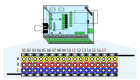
\includegraphics[scale=1]{img/externalPins.pdf}
	\caption{External pins numbering}
	\label{fig:externalPins}
\end{figure}

\begin{table}[H]
	\centering
	\begin{tabular}{|c||c|c|c|c|c|c|c|c|}
		\hline
		& 01 & 02 & 03 & 04 & 05 & 06 & 07 & 08 \\
		\hline \hline
		A & GND & +3V3 & SENSOR\_VP & SENSOR\_VN & IO33 & IO25 & IO32 & IO26 \\
		B & \multicolumn{8}{|c|}{Pins B01 -- B17 internally connected, details in section \ref{jumpersExternalPins}} \\
		C & \multicolumn{8}{|c|}{GND} \\
		\hline
	\end{tabular}

	\vspace{0.5cm}
	
	\begin{tabular}{|c||c|c|c|c|c|c|c|c|c|c|}
		\hline
		& 09 & 10 & 11 & 12 & 13 & 14 & 15 & 16 & 17 & \\
		\hline \hline
		A & IO18 & IO19 & IO21 & IO16 & IO17 & IO23 & IO22 & IO27 & +5V & \\
		B & \multicolumn{10}{|c|}{Pins B01 -- B17 internally connected, details in section \ref{jumpersExternalPins}} \\
		C & \multicolumn{10}{|c|}{GND} \\
		\hline
	\end{tabular}
	\caption{External pins mapping}
	\label{tab:externalPins}
\end{table}

\begin{table}[H]
	\centering
	\begin{tabular}{|c|c|c|c|c|c|}
		\hline
		Number & Name & Safety resistor & Pull-up & Device & Pin \\
		\hline \hline
		01 & GND & N/A & N/A & N/A & N/A \\
		02 & +3V3 & N/A & N/A & N/A & N/A \\
		03 & RADIO\_RX & Yes & No & ESP32 & SENSOR\_VP \\
		04 & RADIO\_TX & Yes & No & ESP32 & SENSOR\_VN \\
		05 & BTN1 & No & Yes & ESP32 & IO33 \\
		06 & BTN0 & No & Yes & ESP32 & IO25 \\
		07 & LED4 & Yes & No & ESP32 & IO32 \\
		08 & SCL0 & Yes & Yes & ESP32 & IO26 \\
		09 & SCK0 & Yes & No & ESP32 & IO18 \\
		10 & MISO0 & Yes & No & ESP32 & IO19 \\
		11 & MOSI0 & Yes & No & ESP32 & IO21 \\
		12 & MPU\_TX & Yes & No & ESP32 & IO16 \\
		13 & MPU\_RX & Yes & No & ESP32 & IO17 \\
		14 & CS\_DECA & Yes & No & ESP32 & IO23 \\
		15 & CS\_MPU2 & Yes & No & ESP32 & IO22 \\
		16 & SDA0 & Yes & No & ESP32 & IO27 \\
		17 & +5V & N/A & N/A & N/A & N/A \\
		\hline
	\end{tabular}
	\caption{External pins properties}
	\label{tab:externalPinsProperties}
\end{table}

\paragraph{Note:} Some external pins are not connected only to processor, but they are connected to other chips in parallel. The other chips are connected only via input only pins or with safety resistor. So, the possibility of damage by incorrect connection or by wrong software is minimized.

\subsection{Pin Description}
\begin{itemize}
	\item 01 -- \textbf{GND}: Ground
	\item 02 -- \textbf{+3V3}: Power Supply \SI{+3.3}{V} from linear stabilizer
	\item 03 -- \textbf{RADIO\_RX}: UART receive pin for external devices like radio communication or GPS
	\item 04 -- \textbf{RADIO\_TX}: UART transmit pin for external devices like radio communication or GPS
	\item 05 -- \textbf{BTN1}: Usage defined by user software, internally connected to button 1
	\item 06 -- \textbf{BTN0}: Usage defined by user software, internally connected to button 0
	\item 07 -- \textbf{LED4}: Usage defined by user software, internally connected to LED4
	\item 08 -- \textbf{SCL0}: \itwoc clock pin for external devices, internally connected to sensors
	\item 09 -- \textbf{SCK0}: SPI clock pin for external devices, internally connected to sensors
	\item 10 -- \textbf{MISO0}: SPI data output pin for external devices, internally connected to sensors
	\item 11 -- \textbf{MOSI0}: SPI data input pin for external devices, internally connected to sensors
	\item 12 -- \textbf{MPU\_TX}: UART transmit pin for GY953 or external device
	\item 13 -- \textbf{MPU\_RX}: UART receive pin for GY953 or external device
	\item 14 -- \textbf{CS\_DECA}: Usage defined by user software, internally used as chip select pin for DWM1000 TDOA location sensor
	\item 15 -- \textbf{CS\_MPU2}: Usage defined by user software, internally connected to GY953 port
	\item 16 -- \textbf{SDA0}: \itwoc data pin for external devices, internally connected to sensors
	\item 17 -- \textbf{+5V}: \SI{+5}{V} power supply from battery or USB or external source, the battery voltage is converted to \SI{5}{V}
\end{itemize}

\paragraph{Note:} All pins except power supply pins can be redefined by software. Their new definition shouldn't be in collision with other connected parts. For details see figures \ref{sch1} and \ref{sch2}.

\subsection{Power Supply}
\label{jumpersExternalPins}
The pins B01 -- B17 are defined by jumpers. We usually need these pins connected to power supply. We can define the voltage by connecting arbitrary B pin to target power supply. The pins B01 -- B17 are internally connected, but they are not connected to anything else. We can define pins B01 -- 17 as:
\begin{itemize}
	\item \textbf{GND} by connecting A01 and B01 by jumper
	\item \textbf{+3V3} by connecting A02 and B02 by jumper
	\item \textbf{+5V} by connecting A17 and B17 by jumper
	\item \textbf{anything} by connecting any B pin to our target
\end{itemize}

\begin{figure}[H]
	\centering
	\includegraphics[scale=1]{img/jumpers.pdf}
	\caption{Power supply definition by jumpers}
	\label{fig:jumpersSupply}
\end{figure}

\section{LED Meanings}

\begin{figure}[H]
	\centering
	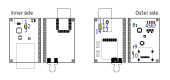
\includegraphics[scale=1]{img/LEDmeanings.pdf}
	\caption{Sensor Board LED meanings}
	\label{fig:LEDmeaning}
\end{figure}

\begin{enumerate}
	\item \textbf{LED\_CBUS3}: (yellow) FTDI LED \cite{FTDI}, USB power indication
	\item \textbf{LED\_CBUS2}: (yellow) FTDI LED \cite{FTDI}, USB connection indication
	\item \textbf{LED\_CBUS4}: (yellow) FTDI LED \cite{FTDI}, USB data transfer indication
	\item \textbf{LED\_5V}: (red) \SI{5}{V} power LED
	\item \textbf{LED\_3V3}: (red) \SI{3.3}{V} power LED
	\item \textbf{LED\_VCCIO}: (red) VCCIO power LED
	\item \textbf{LED\_USB}: (red) USB power LED
	\item \textbf{LED6}: (green) Charging the battery indication
	\item \textbf{LED4}: (green) Software configurable LED
	\item \textbf{LED5}: (green) Software configurable LED
	\item \textbf{LED7}: (yellow) DWM1000 TXLED \cite{DWM1000}
	\item \textbf{LED3}: (yellow) DWM1000 RXLED \cite{DWM1000}
	\item \textbf{LED2}: (yellow) DWM1000 SFDLED \cite{DWM1000}
	\item \textbf{LED1}: (yellow) DWM1000 RXOKLED \cite{DWM1000}
\end{enumerate}

\section{Internal Connections}

\subsection{Internal Pins}
//todo

\begin{figure}[H]
	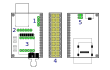
\includegraphics[scale=1]{img/pinSections.pdf}
\end{figure}

\begin{table}[H]
	\begin{tabular}{|c|c|l|}
		\hline
		Number & Usage & Description \\
		\hline
		1 & Internal & BMF055 board connector (UART) \\
		2 & Internal & HM-TRP 433/868 MHz radio connector \\
		3 & Internal & GY-953 connector \\
		4 & External & External pins \\
		5 & Internal & Battery connector \\
		\hline
	\end{tabular}
\end{table}

//todo: detaily ke kazdemu

\subsubsection{BMF055 board connector (UART)}
\subsubsection{HM-TRP 433/868 MHz radio connector}
\subsubsection{GY-953 connector}
\subsubsection{External pins} \ref{pinNumbering}
\subsubsection{Battery connector}

//todo: vyznam testpadu

\section{BMF055 Extension Board}
\label{BMF055pinNumbering}
//todo

\subsection{Pin Connection}
//todo

\subsection{LED Meanings}
//todo



\section{Sensor Board Drawings}
//todo: pridat vedle sebe fotku, render, nakres a eagle brd

\chapter{SensorBoard API documentation}
//todo: add Doxygen export as appendix?


\end{document}
